\chapter{\label{cha:fuzz}Fuzzing}

In this chapter, we describe our high-level algorithm for fuzzing weak memory programs. The next two sections will implement mutations for test generation differently.

\section{Motivation}

As discussed before, weak memory programs can produce nontrivial set of possible executions and testing the program behavior under weak memory models is challenging.
Here is a summary of several characteristics associated with random-based testing for weak memory programs, which we will illustrate with examples:
\begin{itemize}
    \item The program behavior depends not only on scheduling decisions but also weak memory behaviors.
    \item Different scheduling decisions made by the test generator can lead to the same executions. 
    \item The search space of execution graphs is typically large, often larger than in strong memory models.
    \item The probability of finding specific executions is not uniform, with some execution graphs being infrequent.    
\end{itemize}


Firstly, weak memory models usually allow more behaviors which are not permitted in the SC model. For example, under a certain schedule, a read event may have more than one write events to read from. This presents challenges for testing weak memory programs, as their behaviors are not uniquely determined by scheduling decisions. Take SB for example, assuming all operations are relaxed, suppose a tester's scheduler adds events to an execution graph in the following order: \texttt{[$init$]} $\rightarrow$ \texttt{W($x$, 1)} $\rightarrow$ \texttt{W($y$, 1)} $\rightarrow$ \texttt{R($y$)}. When \texttt{R($y$)} is added, it has two reads-from options: \texttt{[$init$]} and \texttt{W($y$, 1)}. This is not possible in the SC model, because under this schedule, \texttt{[$init$]} happens before \texttt{W($y$, 1)}, which in turn happens before \texttt{R($y$)}. Hence, \texttt{R($y$)} can only read from the most recent write in this happen-before order. In the weak memory model, however, since both \texttt{W($y$, 1)} and \texttt{[$init$]} are relaxed, there is no happen-before relationship between them to constrain the read options for \texttt{R($y$)}.

Secondly, different orders of adding events and forming relations can result in the same executions. For example, consider Listing~\ref{P6}, where two groups of threads are incrementing their counters. The test generator might first add events from threads in \texttt{group 1} and then from those in \texttt{group 2}, or it might choose to add events from \texttt{group 2} first. Since the threads in the two groups do not interact with each other, both cases can result in same execution graphs.

% \michalis{Do you need a different example to explain this?}

\begin{lstlisting}[caption={P6}, label={P6}]
    atomic<int> cnt1 = {}; // s0
    atomic<int> cnt2 = {}; // s0
    
    // group 1
    void thread1() { cnt1++; }
    void thread2() { cnt1++; }

    // group 2
    void thread3() { cnt2++; }
    void thread4() { cnt2++; }

\end{lstlisting}


Thirdly, the search space, which is the set of all possible execution graphs, can become very large or even infinite due to various combinations of relations, control flow branches, and loops. For simplicity, assume a single-threaded random test generator is used, which takes one step at a time—either adding a node to the graph or forming a relation between two nodes. Additionally, the test generator has a mechanism to ensure that the steps taken are valid according to the memory model. For example, consider the SB example: if all atomic operations are relaxed, the four execution graphs shown in Figure~\ref{SB4} are all allowed. In thecontrast, under the SC model, only the first three executions are permitted.
% \michalis{This is wrong; 3 graphs are allowed under SC.}


\begin{figure}[h!tbp]  
    \centering
    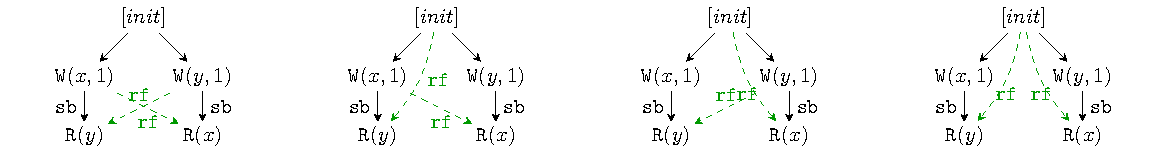
\includegraphics[scale=0.8]{figure/exec-graph/SB4.pdf}   
    \caption{Valid execution graphs of SB}  
    \label{SB4}  
\end{figure}




% Since all loads and stores are relaxed, the loads will have no synchronization constraints. Each load can have 4 possible stores to read from: s0, s1, s2 and s3. Hence the size of the search space is: $4^3 = 64$. Comparing this with the SC model, if all loads and stores are sc, the total number of executions is $\binom{6}{3} = 20$. 




Lastly, the probability of encountering different executions is not uniformly distributed. Some execution graphs are more likely to be found, while others may have a lower probability of being discovered. Consider the example shown in Listing~\ref{P2}, where two threads update their corresponding flags \texttt{x1} and \texttt{x2}, and a third thread reads them. Suppose the test generator makes random decisions uniformly when adding events. The program printing 'A' requires one of the following orders shown in Table~\ref{tab:order-prob}, with a total probability of $\frac{7}{18}$, while printing 'B' has a probability of $\frac{11}{18}$.



\begin{table}[h]
    \centering
    \renewcommand{\arraystretch}{1.5} % 调整行高
    \begin{tabular}{|p{0.3\linewidth}|p{0.3\linewidth}|}    
        \hline
        order & probability  \\ \hline
        \texttt{w1} $\rightarrow$ \texttt{w2} $\rightarrow$ \texttt{r1} $\rightarrow$ \texttt{r2}  & $\frac{1}{3} \times \frac{1}{2} = \frac{1}{6}$ \\  
        \texttt{w2} $\rightarrow$ \texttt{w1} $\rightarrow$ \texttt{r1} $\rightarrow$ \texttt{r2} & $\frac{1}{3} \times \frac{1}{2} = \frac{1}{6}$ \\  
        \texttt{w1} $\rightarrow$ \texttt{r1} $\rightarrow$ \texttt{w2} $\rightarrow$ \texttt{r2} & $\frac{1}{3} \times \frac{1}{3} \times \frac{1}{2} = \frac{1}{18}$    \\ 
        \hline
    \end{tabular}
    \caption{Probabilities of each order}
    \label{tab:order-prob}
\end{table}

\begin{lstlisting}[caption={P2}, label={P2}]
atomic<int> x1 = {};
atomic<int> x2 = {};

void thread1() {
    x1 = 1;     // w1 
}
void thread2() {
    x2 = 1;     // w2
}

void thread3() {
    if(x1 == 1 /* r1 */ && x2 == 1 /* r2 */) {    
        print("A");
        assert(false);
    }
    else {
        print("B");        
    }
}
\end{lstlisting}



The process of the random walk test generation procedure is similar to the Galton board experiment. Consider the following $n$ level decision tree, from top to bottom, each step has two choices, either going left or right. Each node represents a state and the edges represent the decisions. There are some states that can be reached from multiple paths. Take the middle state in the second level for example, it can be reached by first choosing left then right, or by first choosing right then left. There are also some other states that have more strict requirements on the decision making. For example, the state circled in red requires always select the left choices to reach, with the probability of $\frac{1}{2^n}$. 
\begin{figure}[htbp]  
    \centering
    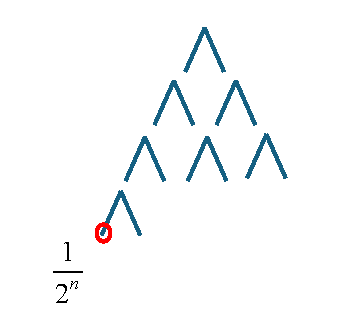
\includegraphics[scale=0.5]{figure/tree.pdf}   
    \caption{Random decision tree}  
    \label{tree}  
\end{figure}



If each time we start from the top and randomly make decisions, those states in the middle will be reached more frequently than those in the corners. However, if we can start from some middle states, it would be easier to reach some corner states, and hence the states reached in the end will be more diverse. This is where our fuzzer come to help. An intuitive description of the fuzzer is: whenever the fuzzer reaches a new state (i.e. finds an interesting execution graph), it mutates one of the decisions made. For the next iteration, the fuzzer replays the decision making until the mutated point, change the decision as mutated, and continues randomly afterwards. As shown in Figure~\ref{tree3} (a), suppose the red path is the previous exploration and the fuzzer mutates the second decision from going right to left (b). Then for the next exploration, it replays until the mutated choice and the probability of reaching the left corner state becomes $\frac{1}{2^{n-2}}$ (c). 

\begin{figure}[h!tbp]  
    \centering
    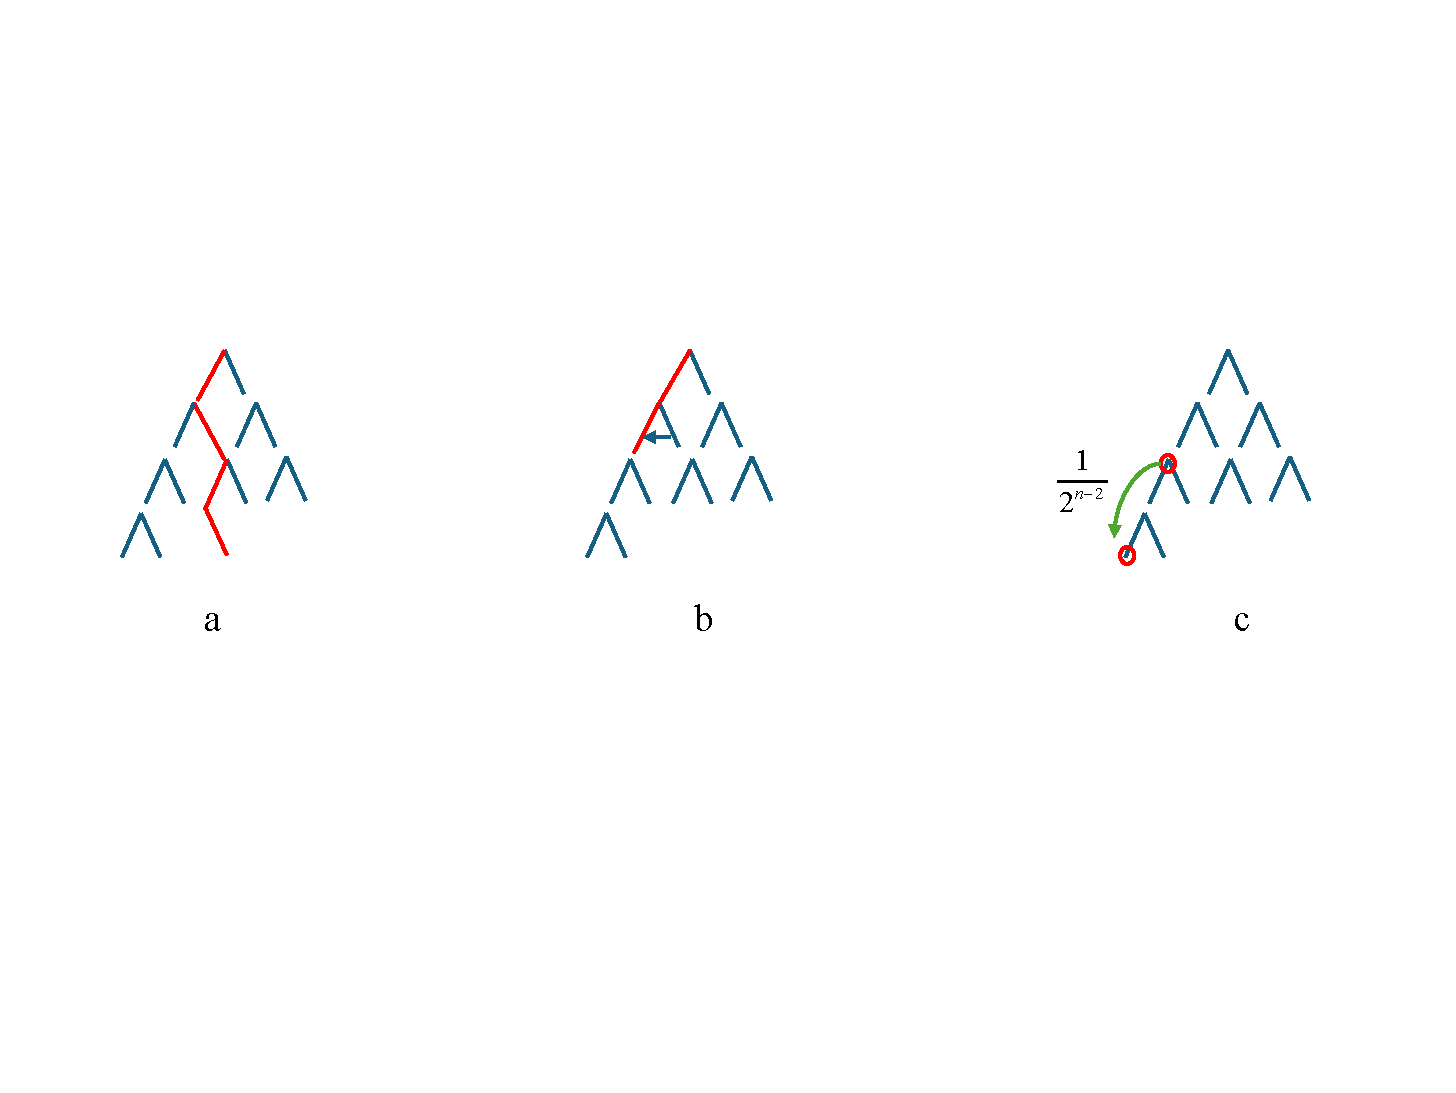
\includegraphics[scale=0.5]{figure/tree3.pdf}   
    \caption{Mutation}  
    \label{tree3}  
\end{figure}

% \michalis{Maybe the example above requires some more explanation. Assuming that a node in your tree is not an execution graph (but rather the rf choices within a graph), can it be the case that two paths yield the same graph? If so, why? If not, why does fuzzing help?}

Relating this to the randomized testing procedure, each parent node in the decision tree represents an intermediate state in the process of constructing a graph, while the leaf nodes represent completed graphs. The edges correspond to the scheduling or rf decisions made during exploration. Each time, the random walk tester restarts from the begining (top of the tree) and randomly generates execution graphs independently. However, due to the previously listed challenges, it often tends to generate a subset of frequently occurring execution graphs, sometimes repeatedly, leaving hard-to-find executions unexplored. We consider this approach inefficient and utilize fuzzing techniques to improve this. Ideally, the fuzzer should explore graphs with a more uniform frequency and broader coverage compared to  the random walk tester, as shown in Figure~\ref{tree-freq}.

\begin{figure}[h!tbp] 
    \centering
    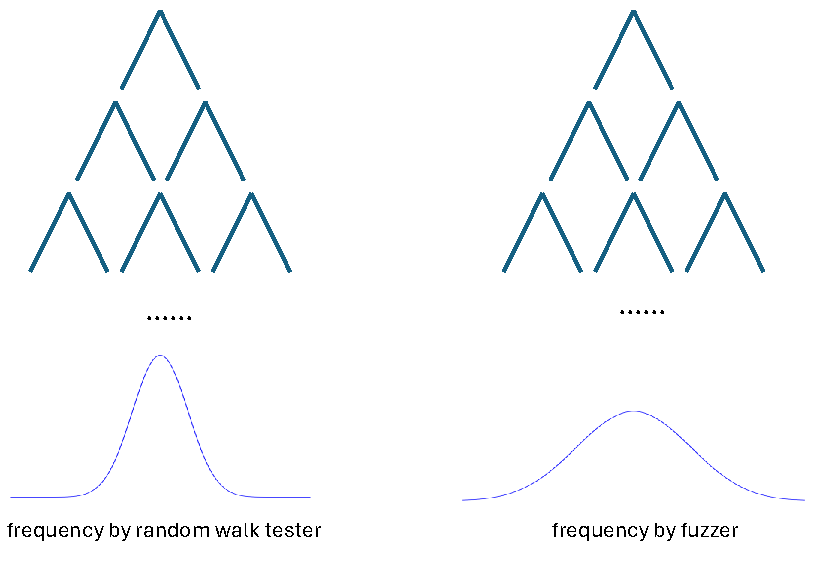
\includegraphics[scale=0.28]{figure/tree_freq.pdf} 
    \caption{Improvement of fuzzing}  
    \label{tree-freq}  
\end{figure}


The fuzzer aims to improve the performance of randomized testing approaches. Some random testers, such as C11Tester or GenMC in its estimation mode, use random walk testing. In contrast, exhaustive model checkers like GenMC explore all possible executions. Exhaustive checkers are useful when the search space is limited, typically when the program under test is not too large. Randomized testers are usually employed for testing larger programs. However, the drawback of this approach is that it does not retain state information between explorations, leading to redundant efforts. In our fuzzing algorithm, we track the explored execution graphs and mutate infrequent ones to guide the tester in covering a larger fraction of the graph search space.

\section{Example}

In this section, we present an example of the fuzzing approach on the execution graphs, using the \ref{exp-fuzz} program with release-acquire pairs. 

\begin{lstlisting}[caption={Fuzzing example}, label={exp-fuzz}]
    atomic<int> x = {};
    
    void thread1() {
        x.store(1, release);    // w1
        x.store(2, release);    // w2
    }
    void thread2() {
        auto r1 = x.load(acquire);    // r1
        auto r2 = x.load(acquire);    // r2
    }
    \end{lstlisting}



Suppose during exploration, one execution graph is constructed as shown in Figure \ref{example_construct}, where the labels of events and relations are omitted. The read values in \texttt{thread2} are both 2. In this execution, \texttt{r2} has only choice to read from, which is \texttt{w2}, since \texttt{r1} has already read from \texttt{w2} and \texttt{r2} reading from w1 will introduce a cycle in the graph. However, \texttt{r1} can have two choices: \texttt{w1} and \texttt{w2}. If the fuzzer consider this execution as interesting and change the rf choice for \texttt{r1}, a new execution can be revealed in the next iteration, as shown in Figure \ref{example_mutate}. 

\begin{figure}[htbp] 
    \centering
    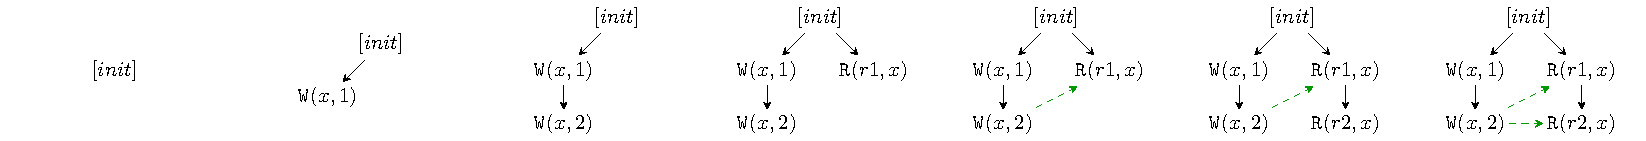
\includegraphics[scale=0.52]{figure/exec-graph/example_construct.pdf} 
    \caption{Construction of an execution graph} 
    \label{example_construct} 
\end{figure}

\begin{figure}[htbp] 
    \centering
    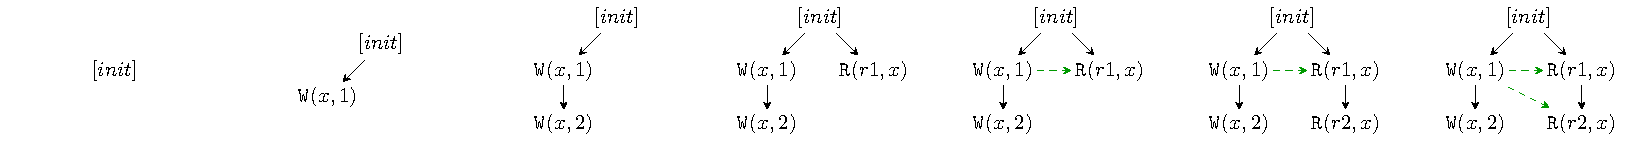
\includegraphics[scale=0.52]{figure/exec-graph//example_mutate.pdf} 
    \caption{Mutate the previous execution graph and re-explore} 
    \label{example_mutate} 
\end{figure}

\michalis{Why can't you get r1 = 1 with testing? A different motivation is required.}
%\burcu{Could you provide an example of the fuzzing approach on the execution graphs? E.g., Give an example program and a random execution graph of the program. Then, show another execution graph that is obtained by some mutation (e.g., mutates the prev. graph after some prefix) and exposes another behavior of the program.}

\section{Overview}


This section provides a high-level overview of the fuzzing algorithm. The implementation details and evaluation results will be presented in later chapters.


The fuzzer uses partially constructed graphs, represented by "prefixes" in the following context, as guidance for further explorations. As shown in Algorithm~\ref{fuzzer}, the fuzzer executes the program $P$ a total of $N$ times (line~\ref{line:input}), generating an execution graph each time after exploring the search space. It maintains a set of prefixes, initially empty (line~\ref{line:init_prefix}). At the beginning of each exploration, it picks a prefix from the prefix set (line~\ref{line:pick_prefix}). If no prefixes are available in the set, the exploration will be entirely random (line~\ref{line:random_explore}). With a selected prefix, the fuzzer replays the execution up to the end of the prefix and randomly constructs the remaining part of the execution graph (line~\ref{line:explore_prefix}). When the exploration is finished, an execution graph is constructed, and the fuzzer determines whether this graph is interesting according to certain metrics (line~\ref{line:is_interesting}). A graph is considered interesting if it is a new execution graph or contains new relations or events. The interesting graph is then mutated to generate new prefixes (line~\ref{line:mutate}). These new prefixes are added to the prefix set for future use (line~\ref{line:add_prefix}). For example, the fuzzer might modify a reads-from relation in the graph and remove the invalid portion following that relation to create a prefix. The fuzzer may also dynamically discard some prefixes based on their effectiveness in finding new interesting graphs. New graphs are added to the graph set (line~\ref{line:add_graph}) and are ultimately outputted at the end (line~\ref{line:output}). 


% \michalis{Why execute only up to N times? Could you do this with a time budget too? If so, mention this.}

\begin{algorithm}
    \caption{Fuzzing algorithm}
    \label{fuzzer}
    \begin{algorithmic}[1]
    \STATE \textbf{Input:} Program $P$ and number of explorations $N$ \label{line:input}
    \STATE \textbf{Output:} $N$ execution graphs
    
    \STATE prefix\_set $\leftarrow \emptyset$ \label{line:init_prefix}
    \STATE graphs $\leftarrow \emptyset$ 
    
    \FOR{$i \leftarrow 1$ \TO $N$}
        \IF{prefix\_set $\neq \emptyset$}   
            \STATE $p \leftarrow$ get\_prefix(prefix\_set) \label{line:pick_prefix}
            \STATE $g \leftarrow $ explore\_from\_prefix($p$) \label{line:explore_prefix}
        \ELSE 
            \STATE $g \leftarrow $ explore\_randomly() \label{line:random_explore}
        \ENDIF 
        \IF{is\_interesting(g)} \label{line:is_interesting}
            \STATE $p' \leftarrow$ mutate(g) \label{line:mutate}
            \STATE prefix\_set $\leftarrow$ prefix\_set $\cup p'$      \label{line:add_prefix}  
        \ENDIF
        \STATE graphs $\leftarrow$ $graphs \cup g$      \label{line:add_graph}
    \ENDFOR
    
    \RETURN graphs      \label{line:output}
    \end{algorithmic}
\end{algorithm}

The following are a few notes regarding this algorithm.

\paragraph*{$N$ as an input parameter} The number of unique execution graphs in the outputted graph set is a major metric for evaluating the fuzzer's searching ability. The algorithm takes a fixed number of iterations, $N$, as an input parameter. This facilitates the comparison of algorithmic efficiencies regardless of implementation details. In practice, execution time is also an important consideration. In our fuzzer implemented with GenMC, described in Chapter~\ref{cha:genmc}, we also evaluate the fuzzer by running it for a fixed time budget and count the number of unique executions found.

% hash 
\paragraph*{Counting the number of unique graphs} In order to count the number of execution graphs, we will also need a hash function that maps the set of graphs, $G$, to a subset of integers, $H$. This hash function, $h: G \to H$ should be a bijection. That is, it should satisfy the following properties:
\begin{itemize}
    \item $h$ is surjective: The same execution graphs should always have the same hash values. This requires the hash function to exclude irrelevant information, such as the timestamps of events. 
	\item $h$ is injective: Different execution graphs should have different hash values. This requires the hash function to include enough information from the graphs. Ideally, there should be no hash collisions, but as this is a low-probability event, it can be ignored within the scope of our work.
\end{itemize}

If $h$ is bijective, the cardinality of the set of hashes, $|H|$, equals that of execution graphs, and can thus be used to count the number of distinct graphs. In our implementations, we use different hash functions due to the differing internals of the C11Tester and GenMC, but both are considered bijective functions.




In the following chapters, we present two fuzzers based on C11Tester and GenMC, both of which implement the fuzzing algorithm, with different implementations for functions such as is\_interesting, mutate,  explore\_from\_prefix and the hash function.


\michalis{Why does it matter whether g is interesting? Isn't it more important that the mutated graph is interesting?}






% \subsection{Threads}





